\documentclass[11pt,aspectratio=43]{beamer}
% BEWARE: IF ASPECTRATIO IS CHANGED YOU NEED TO CHANGE THE PUT COMMAND IN THE HEADER
% (SEE BELOW); for 16:9 and 4:3 values are provided, just un/comment the corresponding lines

% Useful/required packages
\usepackage{amsfonts, amsmath, amssymb, amsthm}
\usepackage{pifont}
\usepackage{multirow}
\usepackage{tikz}
\usetikzlibrary{arrows,calc,decorations.markings,intersections,positioning,shapes.arrows}
\usepackage{epstopdf}
\usepackage{pgfplots}
\usepackage{pgfplotstable}
\pgfplotsset{compat=newest}
\usepackage{booktabs}

\usepackage{textcase}
\usepackage{changepage}
\usepackage{graphicx}
\graphicspath{{img/}{../../doc/images}}

\usepackage{xspace}
\usepackage{stmaryrd}
\usepackage{bm}
% \usepackage{diagbox}

% Pint Algorithms
\newcommand{\Parareal}{\textsc{Para\-real}\xspace}
\newcommand{\PFASST}{\textsc{PFASST}\xspace}
\newcommand{\MGRIT}{\textsc{MGRIT}\xspace}
\newcommand{\RIDC}{\textsc{RIDC}\xspace}
\newcommand{\STMG}{\textsc{STMG}\xspace}

% Parareal
\newcommand{\G}{\mathcal{G}}
\newcommand{\F}{\mathcal{F}}
\newcommand{\Pa}{\mathcal{P}}
\newcommand{\dtF}{\delta t}
\newcommand{\dtG}{\Delta t}
\newcommand{\dtP}{\Delta T}
\newcommand{\GProp}{\underset{t_{n}\rightarrow t_{n+1}}{\G^{\dtG}}}
\newcommand{\FProp}{\underset{t_{n}\rightarrow t_{n+1}}{\F^{\dtF}}}
\newcommand{\ones}{\mbox{1\hspace{-0.2em}I}}

\newcommand{\iInt}[2]{\left\llbracket#1,#2\right\rrbracket}
\newcommand{\iRange}[2]{\left\llbracket#1,#2\right\llbracket}

% Maths notations
\newcommand{\norm}[1]{\left\lVert#1\right\rVert}
\newcommand{\matr}[1]{\mathbf{#1}}
\newcommand{\vect}[1]{\boldsymbol{#1}}
\newcommand{\tvect}[1]{\vec{\vect{#1}}}
\newcommand{\dt}{\Delta t}
\newcommand{\dx}{\Delta x}
\newcommand{\real}{\mathbb{R}}
\newcommand{\compl}{\mathbb{C}}
\newcommand{\infnorm}[1]{\lVert#1\rVert_\infty}
\newcommand{\bigo}{\mathcal{O}}

\newcommand{\Imat}{\matr{I}}
\newcommand{\Qmat}{\matr{Q}}
\newcommand{\QDelta}{\matr{Q}_\Delta}
\newcommand{\Hmat}{\matr{H}}


\newcommand{\uvect}{\vect{u}}
\newcommand{\vvect}{\vect{v}}
\newcommand{\MJac}{\matr{P}_{Jac}}
\newcommand{\MGS}{\matr{\tilde{P}}_{GS}}

\newcommand{\QTilde}{\matr{\tilde{Q}}}
\newcommand{\HTilde}{\matr{\tilde{H}}}
\newcommand{\MJacTilde}{\matr{\tilde{P}}_{Jac}}
\newcommand{\MGSTilde}{\matr{\tilde{P}}_{GS}}
\newcommand{\QDeltaTilde}{\matr{\tilde{Q}}_\Delta}
\newcommand{\TFtoCBar}{\bar{\matr{T}}_F^C}
\newcommand{\TCtoFBar}{\bar{\matr{T}}_C^F}
\newcommand{\TFtoC}{\matr{T}_F^C}
\newcommand{\TCtoF}{\matr{T}_C^F}

\newcommand{\uTilde}{\vect{\tilde{u}}}

%% GFM notations

% Basis
\newcommand{\AMat}{\matr{A}}
\newcommand{\BMat}{\matr{B}}
\newcommand{\DMat}{\matr{D}}
\newcommand{\MMat}{\matr{M}}
\newcommand{\RMat}{\matr{R}}
\newcommand{\eyeMat}{\matr{I}}
\newcommand{\phiOp}{\bm{\phi}}
\newcommand{\chiOp}{\bm{\chi}}

% Approximate operators
\newcommand{\phiApprox}{\bm{\tilde{\phi}}}

% Notations for coarse GFM operators
\newcommand{\CoarseId}{C}
\newcommand{\MCoarse}{M^\CoarseId}
\newcommand{\uCoarse}{\vect{u}^\CoarseId}
\newcommand{\ACoarse}{\matr{A}_\CoarseId}
\newcommand{\chiCoarse}{\bm{\chi}_\CoarseId}
\newcommand{\phiCoarse}{\bm{\phi}_\CoarseId}

% Notations for coarse approximate GFM operators
\newcommand{\phiApproxCoarse}{\bm{\tilde{\phi}}_\CoarseId}

\newcommand{\TMG}{\textsc{TMG}\xspace}
\newcommand{\TMGCoarse}{\textsc{TMG$_c$}\xspace}
\newcommand{\TMGFine}{\textsc{TMG$_f$}\xspace}
\newcommand{\errBnd}{\theta}

% General formating
\newcommand{\eg}{\textit{e.g.}~}
\newcommand{\ie}{\textit{i.e.}~}
\newcommand{\cf}{\textit{cf.}~}

%%% The following allows to cite papers from Bibtex files in footnotes using the \footcite{} command.
%%% To compile, run
%%% >> pdflatex presentation.tex
%%% first (might need to run it twice) and then
%%% >> biber presentation
%%% IMPORTANT: no file extension here! Must be "biber presentation" and not "biber presentation.tex" or "biber presentation.aux"
%%% Then run "pdflatex presentation.tex" again and the reference should show up.
\usepackage[style=authoryear, backend=biber, sorting=none,maxbibnames=50, maxcitenames=8, bibencoding=utf8]{biblatex}
%\renewcommand{\footnotesize}{\tiny}

\setbeamercolor{block title}{use=structure,fg=structure.fg,bg=tuhhcolor!100}
\setbeamercolor{block body}{parent=normal text,use=block title,bg=block title.bg!20!bg}
\setbeamertemplate{blocks}[rounded][shadow]

\setbeamerfont{footnote}{size=\tiny}

% Redefine cite to include journal name (default is only author names + year)
\renewbibmacro*{cite}{%
  \iffieldundef{shorthand}
    {\ifthenelse{\ifnameundef{labelname}\OR\iffieldundef{labelyear}}
       {\usebibmacro{cite:label}%
        \setunit{\addspace}}
       {\printnames{labelname}%
        \setunit{\nameyeardelim}}%
     \usebibmacro{cite:labelyear+extrayear}%
     \setunit{\addcomma\space}%
     \usebibmacro{journal}%
     \usebibmacro{booktitle}%
     }
    {\usebibmacro{cite:shorthand}}}

% This is where you list all Bibtex files you want to use

%%%

% Some useful abbreviations
\newcommand{\R}{\mathbb{R}}
\newcommand{\lossyargs}{(\hat{y},u)}
\newcommand{\half}{\frac{1}{2}}
\newcommand{\halfarg}[1]{\frac{#1}{2}}
\newcommand*{\equal}{=}

% for overlays and painting into pictures
\tikzstyle{every picture} += [remember picture]

% No navigation elements
\beamertemplatenavigationsymbolsempty

% color definitions
\usepackage{xcolor}
\def\muline#1#2{\color{#1}\underline{{\color{black}#2}}\color{black}}

\definecolor{tuhhcolor}{RGB}{46,198,214}
\definecolor{codegreen}{rgb}{0,0.6,0}
\definecolor{codegray}{rgb}{0.5,0.5,0.5}
\definecolor{codepurple}{rgb}{0.58,0,0.82}
\definecolor{backcolour}{rgb}{0.95,0.95,0.92}
\definecolor{deepblue}{rgb}{0,0,0.5}
\definecolor{deepred}{rgb}{0.6,0,0}
\definecolor{deepgreen}{rgb}{0,0.5,0}

% Color declarations
\definecolor{blue_light}{rgb}{0.39,0.39,0.78}
\definecolor{blue_dark}{rgb}{0,0,0.39}
\definecolor{orange_light}{rgb}{0.75,0.41,0.14}
\definecolor{orange_dark}{rgb}{0.39,0.22,0.08}
\definecolor{green_light}{rgb}{0.24,0.47,0.24}
\definecolor{green_dark}{rgb}{0,0.39,0}
\definecolor{red_light}{rgb}{0.78,0.39,0.39}
\definecolor{red_dark}{rgb}{0.6,0.18,0.18}

% these are the colors in the logo, use for highlighting
\definecolor{tuhh_turquoise}{RGB}{45, 198, 214}
\definecolor{tuhh_blue}{RGB}{0, 0, 153}
\definecolor{tuhh_red}{RGB}{134, 0, 22}

\setbeamercolor{normal text}{fg=black!100}
\setbeamercolor{structure}{fg=darkgray!100}
\setbeamercolor{footline}{fg=darkgray!100}


\makeatletter

\def\conference#1{\gdef\@conference{#1}}
\def\insertconference{\@conference}

% Header

% Some magic for the shaded box
\setbeamertemplate{frametitle}{
  \leavevmode%
  \setbox\beamer@tempbox=\hbox{%
    \begin{beamercolorbox}[wd=\paperwidth,ht=5ex]{title}%
        \vbox
        to5ex{\vfil\hbox{\usebeamerfont{structure}\hspace*{2ex}\insertframetitle{}}\vfil}%
    \end{beamercolorbox}%
    }%
  \beamer@tempdim=\ht\beamer@tempbox%
  \advance\beamer@tempdim by 3pt%
  \vskip-\beamer@tempdim%
  \begin{pgfpicture}{5ex}{0pt}{\paperwidth}{50pt}
      \pgfpathrectangle{\pgfpointorigin}{\pgfpoint{\paperwidth}{\beamer@tempdim}}
      \pgfusepath{clip}
      \pgftext[left,base]{\pgfuseshading{beamer@frametitleshade}}
  \end{pgfpicture}
  \vskip-\beamer@tempdim%
  \box\beamer@tempbox%
  \vskip0pt%
	\setlength{\unitlength}{1cm}
	\begin{picture}(15,0)
% TODO: if aspectratio is changed, the coordinates of the logo have to be adjusted
	%\put(13.5,1.45){\makebox(0,0)[t]{
\includegraphics[height=0.9cm]{./tuhh-logo}}}%
	% aspect ratio 16:9
	\put(10.3,1.45){\makebox(0,0)[t]{
\includegraphics[height=0.9cm]{tuhh-logo}}}%
	% aspect ratio 4:3
	\end{picture}
	\vspace{-1cm}
}
% end Header


% Footer

% shaded line separating the footer
\pgfdeclarehorizontalshading[tuhh_turquoise,white]{beamer@frametitleshade}{\paperheight}{%
	color(0pt)=(tuhh_turquoise);
	color(0.75\paperwidth)=(white)}

%%% Footer without red box
%\setbeamertemplate{footline}{
%\pgfdeclarehorizontalshading{myshading}{0.75pt}{color(0pt)=(tuhh_blue); color(0.5\textwidth)=(tuhh_turquoise);color(\textwidth)=(white)}
%\pgfuseshading{myshading}
%\begin{flushleft}
%\hspace*{3ex}
%\insertshorttitle $\quad \mid \quad$ \insertshortauthor
%\hfill
%\insertframenumber%/\inserttotalframenumber
%\hspace*{5ex}
%\end{flushleft}
%}

%% Footer with red box
\setbeamertemplate{footline}{
      \leavevmode%
\setbox\beamer@tempbox=\hbox{%
	\begin{beamercolorbox}[wd=\paperwidth,ht=4ex]{footer}%
		\vbox to4ex{\vfil\hbox to \hsize{\color{white} \bfseries \hspace{3ex} \insertshorttitle{} $\quad \mid \quad$ \insertshortauthor{} \hfil \insertframenumber{} \hspace*{5ex}}\vfil}% %adapt hspace according to author/title length
	\end{beamercolorbox}%
}%
\beamer@tempdim=\ht\beamer@tempbox%
\advance\beamer@tempdim by 3pt%
\vskip-\beamer@tempdim%
\begin{pgfpicture}{5ex}{0pt}{\paperwidth}{50pt}
	\pgfsetfillcolor{red_dark}
	\pgfpathrectangle{\pgfpointorigin}{\pgfpoint{\paperwidth+6ex}{\beamer@tempdim}}
	\pgfusepath{clip,fill}
%	\pgftext[left,base]{\color{red}}
\end{pgfpicture}
\vskip-\beamer@tempdim%
\box\beamer@tempbox%
\vskip0pt%
}
% end Footer

\setbeamersize{text margin left=10pt, text margin right=10pt}

\makeatother

%\AtBeginSection[]
%{
%  \begin{frame}<beamer>
%  \frametitle{Outline}
%  \small
%  \tableofcontents[currentsection]
%  \end{frame}
%}

% TODO: SET INFORMATION HERE
\author[T. Lunet \& J. Hahne]{Jens Hahne (Bergische Universität Wuppertal) \& \underline{Thibaut Lunet}}
\institute{Chair Computational Mathematics\\
	Institute of Mathematics (E-10)\\
	Hamburg University of Technology
}
\title[PinT analysis framework]{
	First steps toward a generic tool for comparing parallel efficiency of \\iterative parallel-in-time algorithms}
\date{February 28, 2023}
\conference{SIAM CSE22 - Amsterdam}  % this non-standard variable/command is
%defined above

\begin{document}

% titlepage
\begingroup % needed to redefine footer locally only for this slide
\setbeamertemplate{footline}{} % no footer on titlepage

% feel free to adjust titlepage as you wish
\begin{frame}{\hspace*{1ex}}
\color{darkgray}

\vspace{3mm}
{\Large \MakeTextUppercase{\inserttitle}\par}

\vspace*{7mm}
{\large\insertauthor}

\vspace*{5mm}
{\footnotesize
\insertinstitute
}

\vspace*{5mm}
\insertconference

\vspace*{3mm}
\insertdate

\end{frame}
\endgroup

\begin{frame}{Main problematic}\vskip3pt
	Current goal of Parallel-in-Time (PinT) methods :\\
	$\Rightarrow$ provide \textbf{additional concurrency} for \textbf{massively parallel} simulations\vskip5pt
	
	Large variety of different PinT algorithms  available :
	\begin{itemize}
		\small
		\item[-] Parareal [Lions, Maday \& Turinici, 2001]
		\item[-] PFASST [Emmett \& Minion, 2012]
		\item[-] MGRIT [Falgout, Friedhoff, Kolev, MacLachlan \& Schroder, 2014]
		\item[-] And many others ...
	\end{itemize}\vskip5pt
	\begin{block}{Current limitations when choosing one approach}
		\begin{enumerate}
			\item Most analysis were done separately
			\item Performance evaluation on different problems
			\item Rely on many different time-stepping schemes
		\end{enumerate}
	\end{block}
	\begin{center}
		\textbf{$\Rightarrow$ need to describe and compare all those methods\\from the same point of view}
	\end{center}
\end{frame}

\begin{frame}{Objectives}
	\textbf{Implement a generic framework analysis tool, allowing to :}
    \begin{enumerate}
        \item[-] write each algorithm using the same notation/formalism
        \item[-] separate algorithm definition from time-stepping method and problem
        \item[-] provide generic convergence bound for each method
        \item[-] generate \textbf{accuracy-based performance models} for each algorithm
    \end{enumerate}\vskip30pt
	
	\textbf{Goal of this presentation :} illustration example
	\begin{enumerate}
		\item Describe the PFASST algorithm in a \textbf{simple formulation ...}
		\item ... that allows to generate a first accuracy-based performance model
		\item (that could be compared to other algorithms ...)
	\end{enumerate}
\end{frame}

\begin{frame}{Common formalism for PinT}\vskip10pt
    \begin{block}{Common factor for each algorithm}
    Iterative PinT algorithms compute an solution of 
    $$
    \begin{pmatrix}
        \bm{\phi} & & &\\
        -\bm{\chi} & \bm{\phi} & &\\
        & \ddots & \ddots &\\
        & & -\bm{\chi} & \bm{\phi}
    \end{pmatrix}
    \begin{bmatrix}
        \uvect_1\\\uvect_2\\\vdots\\\uvect_N
    \end{bmatrix}
    =
    \begin{bmatrix}
        \bm{\chi}(u_0\vect{\ones})\\0\\\vdots\\0
    \end{bmatrix}
    \quad \Leftrightarrow \quad 
    \matr{A}\uvect = \vect{f},$$
    using a given \textbf{iterative method}.
    \end{block}
	$\rightarrow$ sequential time stepping $\Leftrightarrow$ exact solution of the system\vskip20pt
	\textbf{Main goal :} represent PFASST through a block iteration :
	$$
	\uvect^{k+1}_{n+1} = \BMat^0_1(\uvect^k_{n+1})
	+ \BMat^1_0(\uvect^{k+1}_{n}) + \BMat^0_0(\uvect^{k}_{n}) + ...
	$$
\end{frame}

\begin{frame}{Block formulation}\vskip5pt
    \begin{block}{Defining time blocks}
    	\begin{center}
    		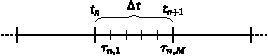
\includegraphics[width=0.6\linewidth]{decompositions.pdf}
    	\end{center}\vskip-10pt
        \begin{enumerate}
            \item $[0,T]$ decomposed into $N$ sub-intervals $[t_n, t_{n+1}]$ of  
            size $\Delta t$
            \item \emph{Block} discretization: $\tau_{n,m} = t_n + \Delta{t}\tau_m,\quad m \in \{1, 2,..., M\}$\\
        \end{enumerate}
    \end{block}
	\begin{itemize}
		\item in our case, $\tau_m$ are the nodes of a collocation method
		\item block variable : $\uvect_n = [u_{n,1}, u_{n,2}, ..., u_{n,M}]^T$
	\end{itemize}\vskip5pt
	\begin{block}{Building block operators}
		Operators mapping two consecutive block variables\vspace{-10pt}
		$$\bm{\phi}(\uvect_{n+1}) = \bm{\chi}(\uvect_{n})
		\quad\Leftrightarrow\quad 
		\uvect_{n+1} = \bm{\phi}^{-1}\bm{\chi}\uvect_{n}
		:= \bm{\psi}(\uvect_{n})$$
	\end{block}	
\end{frame}

\begin{frame}{Collocation and SDC}\vskip3pt
	Collocation method on Dahlquist :\vspace{-10pt}
	$$
	u(t) = u_0 + \int_{0}^{t} \lambda u(\tau)d\tau  \quad
	\Rightarrow \quad
	u(t_n+\tau_m) = u_{n,m} = u_n + \Delta{t}\sum_{j=1}^{M} q_{m,j}\lambda(u_{n,j})
	$$\vspace{-5pt}
	$\Rightarrow$ block formulation (Lobatto nodes) :
	$$(\Imat-\Delta{t}\lambda\Qmat) \uvect_{n} = \begin{pmatrix}
		u_{n,0} \\ \vdots \\ u_{n,0}
	\end{pmatrix} = \Hmat \uvect_{n-1} \quad
	\Rightarrow \quad
	\begin{cases}
		\phiOp = (\Imat-\Delta{t}\lambda\Qmat)\\
		\chiOp = \Hmat
	\end{cases}
	$$\vspace{-10pt}
    \begin{block}{Spectral Deferred Correction (SDC)}
    	1) Built lower triangular approximation $\QDelta$ of dense $\Qmat$ :\vspace*{-3pt}
        $$\phiApprox = (\Imat-\Delta{t}\lambda\QDelta)$$\vskip-3pt
        2) Stationary iteration on collocation system with $\phiApprox$ as preconditionner
    \end{block}\vspace{-25pt}
\end{frame}

\begin{frame}{PFASST in a nutshell}
   	Back to the generic global problem ...
    \begin{equation}\label{eq:globalProblem}
    	\begin{pmatrix}
        \bm{\phi} & & &\\
        -\bm{\chi} & \bm{\phi} & &\\
        & \ddots & \ddots &\\
        & & -\bm{\chi} & \bm{\phi}
    \end{pmatrix}
    \begin{bmatrix}
        \uvect_1\\\uvect_2\\\vdots\\\uvect_N
    \end{bmatrix}
    =
    \begin{bmatrix}
        \bm{\chi}(u_0\vect{\ones})\\0\\\vdots\\0
    \end{bmatrix}
    \quad \Leftrightarrow \quad
    \matr{A}\uvect = \vect{f}
    \end{equation}
    
    \begin{block}{Two-level simplified PFASST}
    Multigrid-based iterative method solving \eqref{eq:globalProblem} with :
    \begin{enumerate}
    	\item One step of an \textit{Approximate Block Jacobi} smoother on a fine level
    	\item One \textit{Approximate Block Gauss-Seidel} iteration on a coarse level \\
    	to estimate the \textit{Coarse Grid Correction}
    \end{enumerate}
    \end{block}
	\textit{See also [Bolten, Moser \& Speck 2017]}\vspace{-20pt}
\end{frame}

\begin{frame}{Approximate Block Jacobi (ABJ)}
	Preconditioned stationary iteration :
	$$\uvect^{k+1} = \uvect^k + \matr{P}_{ABJ}^{-1}(\vect{f}-\AMat\uvect^k) \quad \text{with} \quad 
	\matr{P}_{ABJ} = \begin{pmatrix}
		\phiApprox & & \\
		0 & \phiApprox & \\
		& \ddots & \ddots
	\end{pmatrix}$$
	\begin{block}{Block Iteration}
		\begin{columns}
			\column{0.55\linewidth}\vskip-35pt
			$$\vect{u}_{n+1}^{k+1} = \left[\matr{I} - \tilde{\bm{\phi}}^{-1} \bm{\phi}\right] \vect{u}_{n+1}^{k} +
			\tilde{\bm{\phi}}^{-1}\bm{\chi}\vect{u}_{n}^{k}$$
			
			\column{0.4\linewidth}
			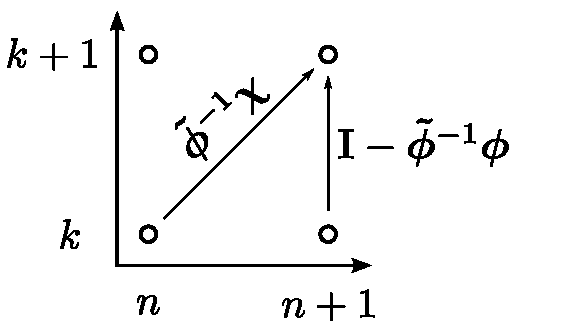
\includegraphics[width=\linewidth]{kn-approxBlockJacobi.pdf}
		\end{columns}
	\end{block}\vspace{-20pt}
\end{frame}

%\begin{frame}{Approximate Block Gauss-Seidel (ABGS)}
%	$$\uvect^{k+1} = \uvect^k + \matr{P}_{ABGS}^{-1}(\vect{f}-\AMat\uvect^k) \quad \text{with} \quad  
%	\matr{P}_{ABGS} = \begin{pmatrix}
%		\phiApprox & & \\
%		-\chiOp & \phiApprox & \\
%		& \ddots & \ddots
%	\end{pmatrix}$$
%	\begin{block}{Block Iteration}
%		\begin{columns}
%			\column{0.55\linewidth}\vskip-35pt
%			$$\vect{u}_{n+1}^{k+1} = \left[\matr{I} - \tilde{\bm{\phi}}^{-1} \bm{\phi}\right] \vect{u}_{n+1}^{k} +
%			\tilde{\bm{\phi}}^{-1}\bm{\chi}\vect{u}_{n}^{k+1}$$
%			
%			\column{0.4\linewidth}
%			\includegraphics[width=\linewidth]{kn-approxBlockGaussSeidel.pdf}
%		\end{columns}
%	\end{block}\vspace{-20pt}
%\end{frame}

\begin{frame}{Coarse Grid Correction (CGC)}
	1) Coarse problem for each block of size $M^C < M$ :
	\begin{equation*}\label{eq:globalCoarseProblem}
		\begin{pmatrix}
			\phiCoarse & & &\\
			-\chiCoarse & \phiCoarse & &\\
			& \ddots & \ddots &\\
			& & -\chiCoarse & \phiCoarse
		\end{pmatrix}
		\begin{bmatrix}
			\uCoarse_{1}\\\uCoarse_{2}\\\vdots\\\uCoarse_{N}
		\end{bmatrix}
		=
		\begin{bmatrix}
			\TFtoC\chiOp(u_0\vect{\ones})\\0\\\vdots\\0
		\end{bmatrix}
		\quad \Leftrightarrow \quad
		\ACoarse\uCoarse = \vect{f}^\CoarseId
	\end{equation*}
	$\rightarrow$ lower order collocation method for $\phiCoarse$ and $\chiCoarse$ ($p$-coarsening)\vskip10pt
	2) $\TFtoC$ and $\TCtoF$ are restriction and prolongation operators (polynomial)\vskip10pt
	3) Standard CGC in global form :
	\begin{align*}
		\ACoarse\vect{d} = \TFtoCBar (\vect{f}-\AMat\uvect^{k})
		&\text{ : coarse grid inverstion}\\
		\uvect^{k+1} = \uvect^{k} + \TCtoFBar\vect{d}
		&\text{ : prolongation + addition on fine level}
	\end{align*}\vspace{-40pt}
\end{frame}

\begin{frame}{ABGS for Coarse Grid Correction}
	4) Approximate CGS with ABGS
	$$
		\tilde{\matr{P}}_{ABGS} \vect{d}^{\ell} =
		(\tilde{\matr{P}}_{ABGS} - \ACoarse)\vect{d}^{\ell-1}
		+ \TFtoCBar (\vect{f}-\AMat\uvect^{k+1/2}),
		\quad \vect{d}^0 = 0,\quad \ell \in \{1,..,L\},
	$$\vspace{-10pt}
	$$
	\ell=1 \quad \Rightarrow \quad \tilde{\matr{P}}_{ABGS} \vect{d} = \TFtoCBar (\vect{f}-\AMat\uvect^{k+1/2}),
	\quad\tilde{\matr{P}}_{ABGS} =
	\begin{bmatrix}
		\phiApproxCoarse & & \\
		- \chiCoarse & \phiApproxCoarse & \\
		& \ddots & \ddots
	\end{bmatrix}
	$$\vspace{-15pt}\\
	5) Simplifying assumptions :
	\begin{enumerate}
		\item $\TFtoC\TCtoF = \Imat$ $\quad\rightarrow\quad$ due to polynomial restriction/prolongation
		\item $\Delta_\chi = \TFtoC\bm{\chi} - \bm{\chi}_C \TFtoC = 0$ $\quad\rightarrow\quad$ due to Lobatto nodes
	\end{enumerate}
	\begin{block}{Block Iteration}
		$$\vect{u}_{n+1}^{k+1} = \left[\matr{I} - \TCtoF\phiApproxCoarse^{-1}\TFtoC\phiOp\right] \vect{u}_{n+1}^{k} +
		\TCtoF\phiApproxCoarse^{-1}\TFtoC\bm{\chi}\vect{u}_{n}^{k+1}$$
	\end{block}\vspace{-20pt}
\end{frame}

\begin{frame}{PFASST as block iteration}
	\begin{columns}
		\column{0.56\linewidth}
		\begin{enumerate}
			\item One ABJ iteration on fine level
			$$\vect{u}_{n+1}^{k+1/2} = \left[\matr{I} - \tilde{\bm{\phi}}^{-1} \bm{\phi}\right] \vect{u}_{n+1}^{k} +
			\tilde{\bm{\phi}}^{-1}\bm{\chi}\vect{u}_{n}^{k}$$
			\item One approximated CGC with ABGS
			\begin{equation*}
				\begin{split}
					\vect{u}_{n+1}^{k+1} 
					&= \left[\matr{I} - \TCtoF\phiApproxCoarse^{-1}\TFtoC\phiOp\right] \vect{u}_{n+1}^{k+1/2} \\
					&~+ \TCtoF\phiApproxCoarse^{-1}\TFtoC\bm{\chi}\vect{u}_{n}^{k+1}
				\end{split}
			\end{equation*}
		\end{enumerate}\vspace{-10pt}
		\begin{block}{Block Iteration}\vskip-10pt
			\begin{equation*}
				\begin{split}
					\uvect_{n+1}^{k+1} &=
					[\eyeMat - \TCtoF\phiApproxCoarse^{-1}\TFtoC \phiOp]
					(\eyeMat - \phiApprox^{-1} \phiOp)\uvect_{n+1}^k \\
					&~+ (\eyeMat - \TCtoF\phiApproxCoarse^{-1}\TFtoC \phiOp)
					\phiApprox^{-1}\chiOp\uvect_{n}^k\\
					&~+ \TCtoF\phiApproxCoarse^{-1}\TFtoC\chiOp\uvect_{n}^{k+1}
				\end{split}
			\end{equation*}
		\end{block}
		
		\column{0.37\linewidth}
		\centering
		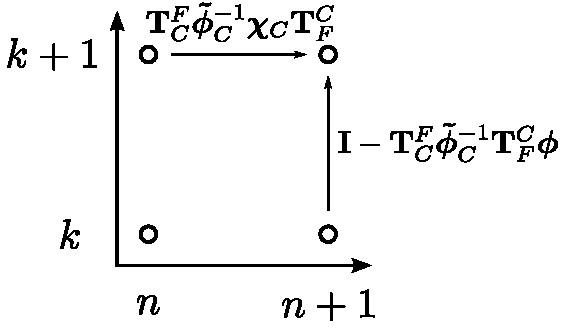
\includegraphics[width=\linewidth]{kn-approxCGC.pdf}
		$$\textbf{+}$$
		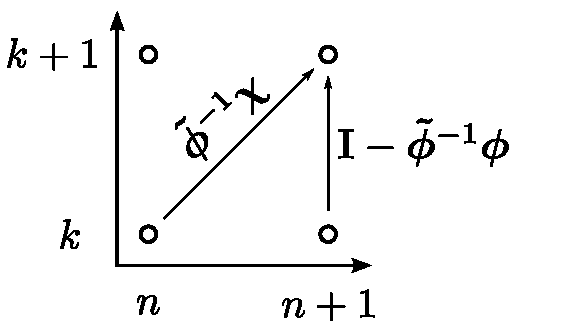
\includegraphics[width=\linewidth]{kn-approxBlockJacobi.pdf}\vspace{-20pt}
	\end{columns}
\end{frame}

\begin{frame}{Task graph}
	\begin{center}
    	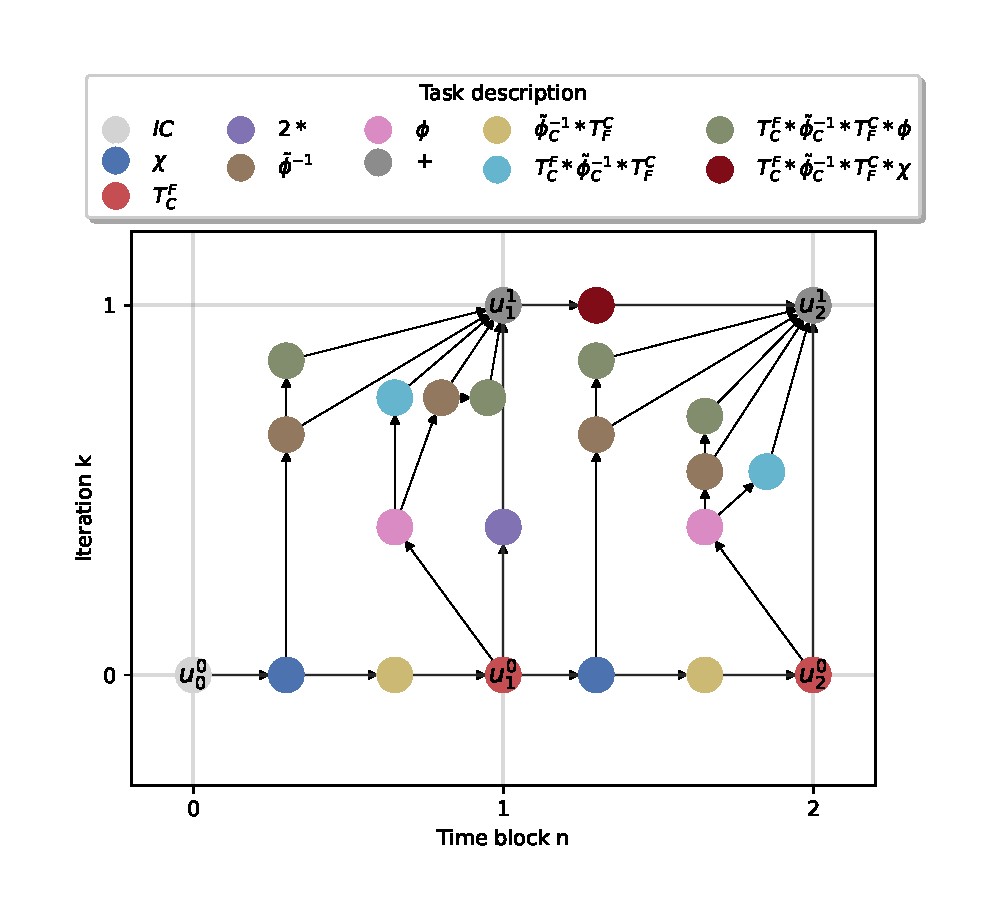
\includegraphics[width=0.6\linewidth]{PFASSTTaskGraph.pdf}
    \end{center}
\end{frame}

\begin{frame}{Task scheduling}
	... TODO ...
\end{frame}

\begin{frame}{Parallel efficiency in the complex plane}
	... TODO ...
\end{frame}

%\begin{frame}{Common formalism for PinT}
%	\begin{block}{Fourth application : PFASST}
%		1) Additional base component : Approximate Block Jacobi
%		\begin{itemize}
%			\item Full matrix representation : 
%			$$\matr{P}_{ABJ} = \begin{pmatrix}
%				\bm{\phiApprox} & & &\\
%				 & \bm{\phiApprox} & &\\
%				&  & \ddots &\\
%				& &  & \bm{\phiApprox}
%			\end{pmatrix}$$
%			$\rightarrow$ still a smoother, but more approximate than BJ\\
%			$\rightarrow$ fully parallel and supposed to be very cheap
%			\item Block Iteration formula :
%			$$\vect{u}_{n+1}^{k+1} = \left[\eyeMat - \phiApprox^{-1} \phiOp\right] \vect{u}_{n+1}^{k} +
%			\phiApprox^{-1}\chiOp\vect{u}_{n}^{k}$$
%		\end{itemize}
%	\end{block}
%\end{frame}

%\begin{frame}{Common formalism for PinT}
%	\begin{block}{Fourth application : PFASST}
%		2) Basic two-level PFASST
%		\begin{enumerate}
%			\item One ABJ iteration : $\vect{u}_{n+1}^{k+1/2} = \left[\eyeMat - \phiApprox^{-1} \phiOp\right] \vect{u}_{n+1}^{k} + \phiApprox^{-1}\chiOp\vect{u}_{n}^{k}$
%			\item One ABGS iteration on coarse level to solve the CGC \\
%			$\rightarrow$ details not shown ...
%		\end{enumerate}\vskip10pt
%		Combination of both produces ...
%		\begin{equation*}
%			\begin{split}
%				\uvect_{n+1}^{k+1} &=
%				[\eyeMat - \TCtoF\phiApproxCoarse^{-1}\TFtoC \phiOp]
%				(\eyeMat - \phiApprox^{-1} \phiOp)\uvect_{n+1}^k \\
%				&~+ (\eyeMat - \TCtoF\phiApproxCoarse^{-1}\TFtoC \phiOp)
%				\phiApprox^{-1}\chiOp\uvect_{n}^k
%				+ \TCtoF\phiApproxCoarse^{-1}\TFtoC\chiOp\uvect_{n}^{k+1}.
%			\end{split}
%		\end{equation*}
%	$\Rightarrow$ \textit{again, simplified description using a Block Iteration}
%	\end{block}
%\end{frame}

\begin{frame}{Conclusion}
	... TODO ...
\end{frame}

\begin{frame}{Acknowledgments}
	\scriptsize\vspace*{-15pt}
	\begin{columns}
		\column[c]{0.5\linewidth}
\includegraphics[width=\linewidth]{EuroHPC.jpg}
		\column[c]{0.2\linewidth}
\includegraphics[width=\linewidth]{logo_eu.png}
		\column[c]{0.3\linewidth}
\includegraphics[width=\linewidth]{BMBF_gefoerdert_2017_en.jpg}
	\end{columns}
	The Time-X project has received funding from the European High-Performance
	Computing Joint Undertaking (JU) under grant agreement No 955701.\\
	The JU receives support from the European Union’s Horizon 2020 research
	and innovation programme and Belgium, France, Germany, and Switzerland.\\
	This project also received funding from the German Federal Ministry of
	Education and Research (BMBF) grant 16HPC048.\vskip10pt	
	\textbf{Partners}
	\begin{columns}
		\column[c]{0.5\linewidth}
		\begin{itemize}
			\item Bergische Universität Wuppertal (BUW)
			\item Ecole des Ponts ParisTech (ENPC)
			\item Forschungszentrum Jülich (FZJ)
			\item Katholieke Universiteit Leuven (KUL)
			\item Sorbonne Université (SU)
		\end{itemize}
		\column[c]{0.5\linewidth}
		\begin{itemize}
			\item Technische Universität Darmstadt (TUD)
			\item Technische Universität Hamburg (TUHH)
			\item Technische Universität München (TUM)
			\item Università della Svizzera italiana (USI)
			\item Université de Genève (UNIGE)
		\end{itemize}
	\end{columns}
	\vspace*{-35pt}
\end{frame}

\appendix

\begin{frame}{Parareal}
	\begin{block}{Block iteration components}
		\begin{enumerate}
			\item One BJ iteration ($\omega=1$) : $\uvect_{n+1}^{k+1/2} = \bm{\phi}^{-1}\bm{\chi} \uvect_{n}^k$
			\item One ABGS iteration : $\uvect_{n+1}^{k+1} = [\matr{I} - \bm{\phiApprox}^{-1}\bm{\phi}]\uvect_{n+1}^{k+1/2} + \bm{\phiApprox}^{-1}\bm{\chi} \uvect_{n}^{k+1}$
		\end{enumerate}
	\end{block}\vskip10pt
	Combination of both produces ...
	$$\uvect_{n+1}^{k+1} = [\bm{\phi}^{-1}\bm{\chi} - \bm{\phiApprox}^{-1}\bm{\chi}]\uvect_{n}^k + \bm{\phiApprox}^{-1}\bm{\chi} \uvect_{n}^{k+1}$$
	... which is the update formula of Parareal :
	$$\uvect_{n+1}^{k+1} = \mathcal{F}(\uvect_{n}^k) + \mathcal{G}(\uvect_{n}^{k+1}) - \mathcal{G}(\uvect_{n}^{k})$$
	$$ \mathcal{F} = \bm{\phi}^{-1}\bm{\chi}, \quad \mathcal{G} = \bm{\phiApprox}^{-1}\bm{\chi}$$
	\begin{center}
		\textit{Not a surprise, since Parareal was built as a block iteration ...}
	\end{center}
\end{frame}

\begin{frame}{MGRIT with FCF-relaxation}
	\begin{block}{Block iteration components}
		\begin{enumerate}
			\item Two BJ iterations : $\uvect_{n+1}^{k+1/2} = \bm{\phi}^{-1}\bm{\chi} \uvect_{n}^k$, 
			$\quad\uvect_{n+1}^{k+1/3} = \bm{\phi}^{-1}\bm{\chi} \uvect_{n}^{k+1/2}$
			\item One ABGS iteration : $\uvect_{n+1}^{k+1} = [\matr{I} - \bm{\phiApprox}^{-1}\bm{\phi}]\uvect_{n+1}^{k+1/3} + \bm{\phiApprox}^{-1}\bm{\chi} \uvect_{n}^{k+1}$
		\end{enumerate}
	\end{block}
	\vskip10pt
	Combination of both produces ...
	$$\uvect_{n+1}^{k+1} = [\bm{\phi}^{-1}\bm{\chi} - \bm{\phiApprox}^{-1}\bm{\chi}]\bm{\phi}^{-1}\bm{\chi}\uvect_{n}^k 
	+ \bm{\phiApprox}^{-1}\bm{\chi} \uvect_{n}^{k+1}$$
	... which is the update formula of overlapping variant of Parareal :
	$$\uvect_{n+1}^{k+1} = \mathcal{F}\circ\mathcal{F}(\uvect_{n}^k) + \mathcal{G}\circ\mathcal{F}(\uvect_{n}^{k+1}) - \mathcal{G}(\uvect_{n}^{k})$$
	$$ \mathcal{F} = \bm{\phi}^{-1}\bm{\chi}, \quad \mathcal{G} = \bm{\phiApprox}^{-1}\bm{\chi}$$
	\begin{center}
		\textit{Equivalence was already proven in [Gander, Kwok and Zhang, 2018]}
	\end{center}
\end{frame}

\end{document}